\section{Geospatial web application}
The geospatial application is located at directory 'geo', consisting of 2 parts, visualization and display.  

\begin{figure}[h]
\centering
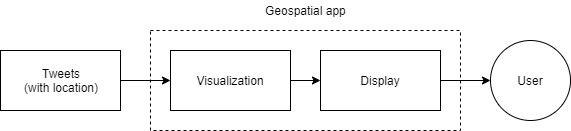
\includegraphics[width=0.7\textwidth]{geoapp}
\caption{Geospatial application}
\end{figure}

The application is set to run 24/7, keeping the visualizations updated with constantly arriving tweet data. In this project, our geospatial statistics are based on Statistical Areas Level 4 (SA4) in Australia. The boundary map can be downloaded from the \href{https://www.abs.gov.au/}{Australian Bureau of Statistics} website.  

\subsection{Visualization}
Tweet data (with location) is fetched directly from CouchDB database, then aggregated to obtain the statistics of interest. The IP address of the host, required for accessing the databases, can be parsed from the auto-generated inventory file, according to the host's name.  

The statistical data is visualized by laying a second layer of different colors on top of the base map. Any map or graph generated is saved on disk, ready to be displayed in a web browser.  

\subsection{UI design}
\subsubsection{Web application}
A simple web application is designed to visualize our data and scenarios. Since Python is used across our project, we choose to use Flask for web development. Flask is a lighter weight framework for Python. It can provide an interaction between the web application and the database, as well as the file system. In our web application, we are going to use two maps and two charts to display our data. Our backend application will automatically collect the data from couchDB and generate the maps and charts as static .html files. After that, our Flask application will render these templates and include them in one frame on our front-end web page. Four buttons are designed to switch between these templates with the help of some JavaScript functions. The Flask application will also play the role of a data retriever of our database. While running, it will continuously read the data from couchDB and present them on the front-end web page. We have manually selected 3 sets of data to display, which are updated frequently, to show that our web application can real-time update the data. A window showing the tweets from the Department of Health of Australian Government. 

\begin{figure}[h]
\centering
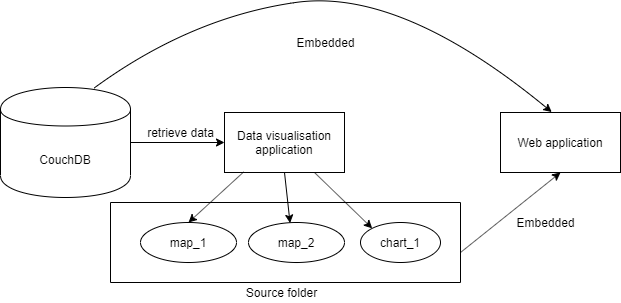
\includegraphics[width=0.7\textwidth]{front-back-end}
\caption{front-back-end interaction}
\end{figure}

\subsubsection{Future extensions}
This web application is easy to extend to have other features. Since its back-end is connected to couchDB, we can access any data we have. For example, the number of positive tweets in one particular area. Hence we will also be able to add a search feature, in which users can select preferred data from a given list and the web will return the required data. In this way, it allows interaction between users and our database. Some other functions can also be achieved with appropriate JavaScript libraries. For example, some data visualisation libraries can be used to plot dynamic charts from data, so that users can see auto-generated charts instead of a bunch of numbers.

\subsubsection{Limitations and challenges}
Flask has many limitations while using it for bigger applications. If our web application scales up to a large website, it will not be able to handle the huge amount of requests because the server is single-threaded. It will become very slow. If it has other responsibilities, in our case being a data retriever, it can get much slower. 
One of the challenges we faced using slack is the use of static files. As mentioned above, we need to embed two charts in image form into our web application. Hence we embedded them as static files. However, the images will be replaced periodically by new images generated by the back-end application but the old images are already recorded in the cache of the web browser. This means sometimes we can’t see the real-time updated charts in our web application although they are already updated. One possible solution is to cache control codes to the header of our web page, ensuring that it will reload the images every time we refresh the page. It may take some extra time, but that situation can be avoided.
